\documentclass[11pt]{article}

\usepackage[review]{acl}

\usepackage{times}
\usepackage{latexsym}
\usepackage[T1]{fontenc}
\usepackage[utf8]{inputenc}
\usepackage{microtype}
\usepackage{inconsolata}
\usepackage{graphicx}
\usepackage{amsmath}
\usepackage{amssymb}
\usepackage{booktabs}
\usepackage{multirow}
\usepackage{xcolor}
\usepackage{subcaption}
\usepackage{algorithm}
\usepackage{algorithmic}

\newcommand{\styleshield}{\textsc{StyleShield}}
\newcommand{\langflow}{\textsc{LangFlow}}
\newcommand{\pai}{P_{\text{AI}}}
\newcommand{\gammavar}{\gamma}

\title{\styleshield{}: Continuous and Controllable Style Transfer \\
for Evading AI-Generated Content Detectors}

\author{Anonymous}

\begin{document}
\maketitle

\begin{abstract}
    AI-generated content (AIGC) detectors are increasingly deployed in 
    high-stakes settings such as academic integrity screening, yet their 
    reliability rests on a fundamental paradox: language models are trained 
    on human-written corpora, so the statistical boundary between AI and 
    human writing will inevitably dissolve as models improve. Commercial 
    incentives have further distorted this landscape---detection and 
    ``de-AIification'' services often operate within the same supply chain, 
    replacing evaluation of content quality with judgment of content origin.
    We present \styleshield{}, the first flow matching framework for 
    \emph{conditional} text style transfer, operating directly in continuous 
    token embedding space via a DiT backbone with zero-initialized 
    cross-attention adapters conditioned on frozen Qwen-7B representations. 
    At inference, we adapt the SDEdit paradigm to text embeddings, with a 
    single parameter $\gamma$ providing smooth continuous control over the 
    evasion--preservation trade-off---fundamentally inaccessible to 
    discrete-token methods. On a multi-domain Chinese benchmark, 
    \styleshield{} at $\gamma{=}7.0$ achieves 94.6\% evasion against the 
    training detector and $\geq$99\% against three unseen detectors, 
    maintaining 0.928 semantic similarity, substantially outperforming 
    backtranslation, synonym substitution, and LLM rewriting baselines. 
    We further propose \emph{RateAudit}, a diagnostic algorithm
    that demonstrates how document-level detection rates can be
    shifted to arbitrary pre-specified values, directly
    questioning the trustworthiness of score-based verdicts.
    \end{abstract}
\section{Introduction}
\label{sec:intro}

The rapid proliferation of large language models (LLMs) has given rise to a burgeoning industry of AI-generated content (AIGC) detectors~\citep{he2023mgtbench, mitchell2023detectgpt, yang2024survey}.
These tools are now deployed at scale in academic institutions, publishing platforms, and content moderation pipelines, where a positive detection result can carry serious consequences---from academic penalties to content removal.
Yet this rush to detect has outpaced our understanding of what, exactly, is being measured.

\paragraph{The Detection Fallacy.}
We argue that the prevailing detector paradigm rests on a fundamentally unstable foundation.
First, \textbf{the boundary between AI and human text is inherently blurring}: modern LLMs are trained on human-written corpora, and humans increasingly incorporate AI suggestions into their writing workflows.
The stylistic features that detectors exploit---perplexity patterns, vocabulary distributions, syntactic regularity---reflect tendencies, not categorical distinctions.
Second, \textbf{commercial incentives distort the landscape}: detection services profit from flagging content as AI-generated, creating systemic bias toward false positives with little accountability for the consequences.
Third, \textbf{detector reliability is poor in practice}: \citet{sadasivan2023aigenerated} demonstrate that paraphrasing attacks can reduce detection accuracy to near-chance, and cross-domain generalization remains weak~\citep{he2023mgtbench}.
These observations suggest that judging text by its \emph{origin} rather than its \emph{quality} is both technically fragile and philosophically misguided.

\paragraph{Limitations of Existing Evasion Methods.}
Prior work on evading AIGC detectors has explored several directions, each with significant drawbacks:
(1)~\textbf{LLM rewriting} asks another language model to paraphrase the text, but the output often retains or even amplifies characteristic AI patterns (we observe near-zero evasion rates on strong detectors);
(2)~\textbf{backtranslation} via machine translation introduces semantic drift and unnatural phrasing, achieving moderate evasion at the cost of substantial quality degradation;
(3)~\textbf{synonym substitution} makes only surface-level lexical changes that barely perturb detector confidence.
Critically, none of these methods offers \emph{continuous control} over the degree of style transformation---users face a binary choice between the original text and a single, opaque rewrite.

\paragraph{Our Approach.}
We propose \styleshield{}, a flow-matching-based framework that treats AI-to-human style transfer as a \emph{continuous denoising process}.
Our key insight is that the SDEdit paradigm~\citep{meng2022sdedit}---adding noise to input data and denoising with a pretrained generative model---can be adapted from images to token embeddings, enabling smooth, controllable style transfer in the continuous embedding space.

Concretely, \styleshield{} builds on a Diffusion Transformer (DiT) backbone pretrained with flow matching on Chinese text~(\langflow{}).
We augment each DiT block with a \textbf{cross-attention adapter} that attends to frozen hidden states from a Qwen-7B encoder~\citep{qwen2024qwen25}, injecting semantic awareness that preserves the meaning of the source text during denoising.
These adapters are zero-initialized so the model starts equivalent to the pretrained \langflow{} and gradually learns to incorporate conditioning.
A \textbf{detector-in-the-loop reward} signal, derived from a BERT-based AIGC detector, provides targeted training feedback that sharpens evasion capability.
At inference, a single parameter~$\gamma$ controls the noise level and hence the intensity of style transformation, enabling users to navigate the Pareto frontier between evasion strength and semantic preservation.

\paragraph{Contributions.}
Our main contributions are:
\begin{enumerate}
    \item We introduce \styleshield{}, the first flow-matching framework for continuous, controllable AI-to-human text style transfer, achieving state-of-the-art evasion rates ($\geq$90.6\% on the training detector, $\geq$99\% on unseen detectors) while preserving high semantic similarity (0.928) on a 1{,}000-sample multi-domain benchmark.
    \item We propose a cross-attention conditioning mechanism with zero-initialized adapters that injects frozen LLM representations into a DiT backbone, enabling semantics-aware denoising without fine-tuning the LLM.
    \item We design an allocator algorithm for long-document style transfer with precise, user-specified detection rate targets, and provide comprehensive ablation studies validating each architectural component.
\end{enumerate}

\section{Related Work}
\label{sec:related}

\paragraph{AIGC Detection.}
Supervised AIGC detectors, typically BERT-based classifiers trained
on human/machine text corpora~\citep{devlin2019bert, he2023mgtbench},
are complemented by zero-shot methods exploiting probability
curvature~\citep{mitchell2023detectgpt} or
watermarking~\citep{kirchenbauer2023watermark}.
However, \citet{sadasivan2023aigenerated} show that simple
paraphrasing dramatically reduces detection accuracy, and
cross-domain transfer remains
fragile~\citep{he2023mgtbench, yang2024survey}.

\paragraph{Text Style Transfer and Adversarial Probing.}
Style transfer methods---variational autoencoders, back-translation,
retrieve-and-edit pipelines, and LLM
rewriting~\citep{lyu2021style}---all operate on discrete tokens and
cannot continuously modulate transformation intensity.
Token-level adversarial attacks such as
TextFooler~\citep{jin2020bert} flip classifier predictions through
lexical substitution but likewise lack continuous controllability.
\citet{krishna2024paraphrasing} show that paraphrasing can evade
detectors, though retrieval-based defenses offer partial mitigation.
All prior methods thus lack a continuous diagnostic axis over
transformation intensity---a capability that continuous
embedding-space generation uniquely affords.

\paragraph{Diffusion and Flow Matching for Text.}
\citet{li2022diffusion} propose Diffusion-LM for controllable
generation in embedding space; \citet{lou2024discrete} develop MDLM
for discrete diffusion. \citet{chen2026langflow} show that continuous
flow matching rivals discrete diffusion in language modeling.
Existing methods address unconditional or class-conditional
generation; source-conditioned style transfer remains
unexplored---a gap \styleshield{} fills.
\section{Method}
\label{sec:method}

\begin{figure}[t]
    \centering
    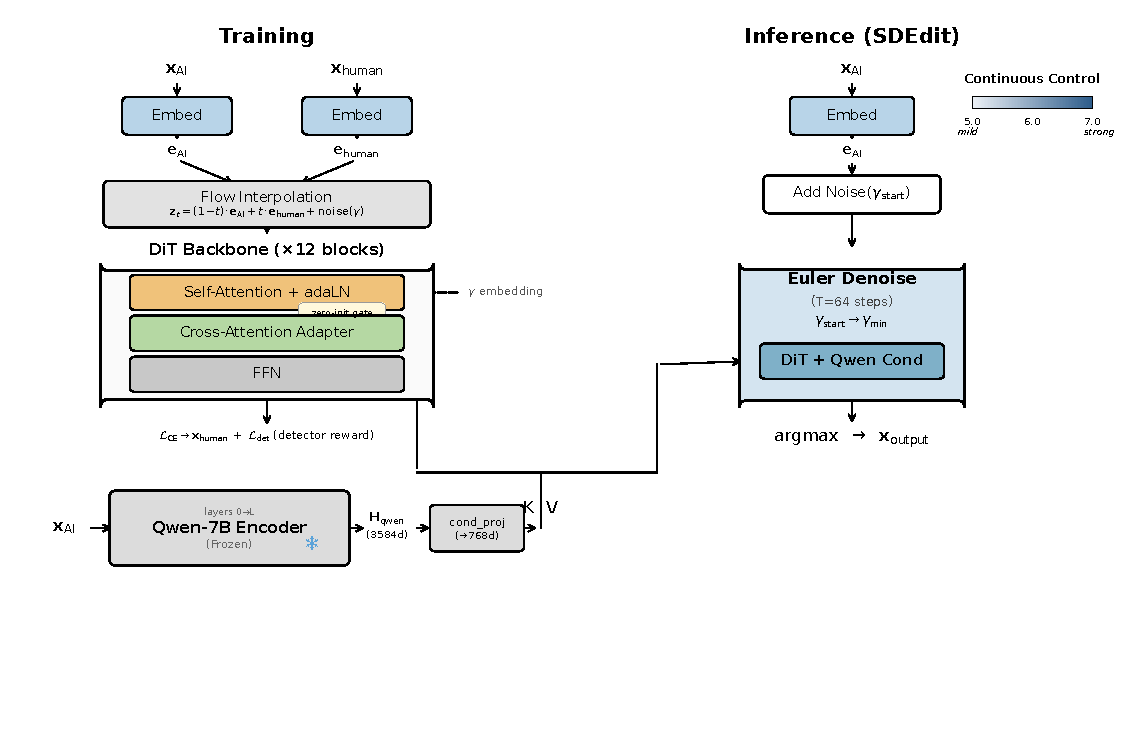
\includegraphics[width=\columnwidth]{figures/fig1_architecture.pdf}
    \caption{Overview of \styleshield{}.
    A pretrained DiT backbone (left) is augmented with zero-initialized
    cross-attention adapters that attend to frozen Qwen-7B hidden
    representations (bottom).
    At inference (right), AI text embeddings are noised at level~$\gamma$
    and iteratively denoised with semantic conditioning via 64 Euler steps.
    The single parameter~$\gamma$ serves as a continuous
    diagnostic axis for characterizing the
    evasion--preservation trade-off.}
    \label{fig:architecture}
\end{figure}

We present \styleshield{}, a conditional flow-matching framework
that operates in continuous token-embedding space, designed as
an adversarial diagnostic for probing AIGC detector robustness.
The system has three components: a DiT backbone pretrained with
flow matching (\S\ref{sec:backbone}), cross-attention adapters
conditioned on a frozen Qwen encoder
(\S\ref{sec:conditioning}), and a training pipeline with
detector-in-the-loop feedback (\S\ref{sec:training}).
At inference a single parameter~$\gamma$ provides continuous
control over transformation intensity, serving as a diagnostic
axis for characterizing detector sensitivity
(\S\ref{sec:inference}).
We further describe \textbf{RateAudit}, a document-level
scheduling algorithm that stress-tests whether detection-rate
verdicts can be set to arbitrary values
(\S\ref{sec:allocator}).
Figure~\ref{fig:architecture} shows the overall architecture.

%% ────────────────────────────────────────────────────
\subsection{Flow Matching Backbone}
\label{sec:backbone}

\styleshield{} operates in continuous token-embedding space via
a Diffusion Transformer
(DiT;~\citealp{peebles2023scalable}) trained with the flow
matching objective~\citep{lipman2023flow, karras2022elucidating}.

\paragraph{Embedding space.}
Each token~$w_i$ is mapped to a $d$-dimensional embedding
$\mathbf{e}_i \in \mathbb{R}^d$ ($d{=}768$) via a learned
vocabulary embedding layer.
Embeddings are length-normalized to stabilize training in the
continuous space:
$\bar{\mathbf{e}} = \sqrt{d}\;\mathbf{e}/\|\mathbf{e}\|$.

\paragraph{Architecture.}
The DiT consists of $N{=}12$ transformer blocks with
self-attention (RoPE), FFN (GELU, expansion ratio~4), and
adaLN-Zero conditioning.
A timestep embedder maps~$\gamma$ to
$\mathbf{c}_\gamma$, which modulates each block:
\begin{equation}
    \mathbf{x}'
      = (1 + \mathbf{s}_\gamma)
        \odot \mathrm{LN}(\mathbf{x})
        + \mathbf{b}_\gamma
\end{equation}
where $\mathbf{s}_\gamma, \mathbf{b}_\gamma$ are predicted from
$\mathbf{c}_\gamma$ via a zero-initialized linear layer.
We additionally employ a bias skip
connection~\citep{karras2022elucidating}:
\begin{equation}
    \mathrm{logits}
      = f_\theta(\mathbf{z},\gamma)
        + c_{\mathrm{skip}}(\gamma)
          \;\mathbf{z}\,\mathbf{W}_{\mathrm{emb}}^\top
\end{equation}
where
$c_{\mathrm{skip}}(\gamma)
  = \exp\bigl((\mathrm{softplus}(-\gamma)-\gamma)/2\bigr)$
provides a direct residual path from the noisy input to the
output logits, stabilizing training at low noise levels.

\paragraph{Noise schedule and Gumbel proposal.}
Following the EDM formulation~\citep{karras2022elucidating},
the forward noising process at noise level~$\gamma$ is:
\begin{equation}
    \mathbf{z}_\gamma
      = \alpha(\gamma)\,\mathbf{x}
      + \sigma(\gamma)\,\boldsymbol{\epsilon},
    \quad
    \boldsymbol{\epsilon}\sim\mathcal{N}(\mathbf{0},\mathbf{I})
    \label{eq:noise}
\end{equation}
where $\alpha(\gamma) = \sqrt{\mathrm{sigmoid}(-\gamma)}$ and
$\sigma(\gamma) = \sqrt{\mathrm{sigmoid}(\gamma)}$.
During training, noise levels are sampled from a learned Gumbel
proposal
$\gamma \sim \mathrm{Gumbel}(\mu, \beta)$.

%% ────────────────────────────────────────────────────
\subsection{Cross-Attention Conditioning}
\label{sec:conditioning}

Style transfer, unlike unconditional generation, must preserve
the semantic content of a \emph{specific} input text.
We inject this content signal via cross-attention adapters
conditioned on a frozen large language model.

\paragraph{Semantic encoder.}
We use Qwen-2.5-7B-Instruct~\citep{qwen2024qwen25} as a frozen
feature extractor.
The AI-text input is tokenized with the Qwen tokenizer and
passed through layers~$0$ to~$L{-}1$
(default $L{=}14$ of 28); the resulting hidden states
$\mathbf{H}_{\mathrm{qwen}}
  \!\in\! \mathbb{R}^{B \times S_q \times 3584}$
encode the semantic content to be preserved.
A learned projection
$\mathrm{proj}\!:\!\mathbb{R}^{3584}{\to}\mathbb{R}^{768}$
maps Qwen features to the DiT hidden dimension.
The Qwen model is kept entirely frozen throughout training---no
gradients flow through it.
The choice of split layer~$L$ trades surface-level fidelity
against semantic abstraction; we ablate
$L\!\in\!\{7,14,21\}$ in \S\ref{sec:ablation}, finding
$L{=}14$ optimal.

\paragraph{Adapter architecture.}
After each DiT self-attention block we insert a
\textbf{cross-attention adapter}.
Each adapter performs multi-head cross-attention where queries
come from the flow tokens and keys/values come from the
projected Qwen hidden states:
\begin{align}
    \mathbf{Q} &= \mathbf{W}_q\;\mathrm{LN}(\mathbf{x}),
    \quad
    [\mathbf{K};\mathbf{V}]
      = \mathbf{W}_{kv}\;\mathrm{proj}(\mathbf{H}_{\mathrm{qwen}})
    \label{eq:cross-kv}\\[2pt]
    \mathbf{x}'
      &= \mathbf{x}
       + \underbrace{g(\mathbf{c}_\gamma)}_{\text{zero-init gate}}
         \!\odot\;
         \mathrm{MHA}(\mathbf{Q},\mathbf{K},\mathbf{V})
    \label{eq:cross-gate}
\end{align}
The gate
$g(\mathbf{c}_\gamma)
  = \mathbf{W}_g\,\mathbf{c}_\gamma + \mathbf{b}_g$
is initialized to zero
($\mathbf{W}_g{=}\mathbf{0},\;\mathbf{b}_g{=}\mathbf{0}$).
This zero initialization is critical: at the start of training,
the adapters have no effect ($g \equiv \mathbf{0}$), so the
model is exactly the pretrained backbone.
The gates gradually open as training progresses, allowing the
model to smoothly learn to incorporate semantic conditioning
without catastrophic forgetting of the pretrained generative
capability.
Each adapter adds $\sim$4$d^2$ parameters per block
($\sim$28M total across 12~blocks), a modest overhead.

%% ────────────────────────────────────────────────────
\subsection{Training}
\label{sec:training}

\paragraph{Data construction.}
We construct 436K parallel (AI, human) text pairs across three
Chinese-language domains---social media (346K), news (68K), and
academic abstracts (22K).
For each domain, we collect human-written texts and prompt
Qwen-2.5-7B-Instruct to rewrite them into AI style.
Each pair is then scored by the AIGC detector and subjected to
\textbf{dual-end strict filtering}: we retain only pairs where
the human side scores $\pai < 0.1$ and the AI side scores
$\pai > 0.9$, ensuring a clean stylistic separation between
the two ends of every training pair.

\paragraph{Denoising objective.}
Given a pair $(x_{\mathrm{AI}}, x_{\mathrm{hu}})$, we embed
both texts, sample $t\!\sim\!\mathcal{U}(0,1)$ and~$\gamma$
from the Gumbel proposal, form the noisy input via flow
interpolation
$\mathbf{z}
  = (1{-}t)\,\mathbf{e}_{\mathrm{AI}}
  + t\,\mathbf{e}_{\mathrm{hu}}$
followed by noise corruption (Eq.~\ref{eq:noise}), and
minimize the denoising cross-entropy:
\begin{equation}
    \mathcal{L}_{\mathrm{CE}}
      = -\!\sum_{i=1}^{S}
          \log\, p_\theta\!\bigl(
            w_i^{\mathrm{hu}}
            \;\big|\;
            \mathbf{z}_\gamma,\; \gamma,\;
            \mathbf{H}_{\mathrm{qwen}}
          \bigr)
    \label{eq:ce}
\end{equation}
The Qwen condition $\mathbf{H}_{\mathrm{qwen}}$ is computed
from~$x_{\mathrm{AI}}$; thus the model learns to denoise
toward the human target while attending to the source semantics.

\paragraph{Detector-in-the-loop reward.}
After a 5{,}000-step warmup we introduce an auxiliary
adversarial signal from a frozen BERT-based AIGC detector.
Periodically, we run inference on a training batch, score the
outputs, and add a reward term:
\begin{equation}
    \mathcal{L}
      = \mathcal{L}_{\mathrm{CE}}
      + \lambda_{\mathrm{det}}\;
        \pai\!\bigl(\hat{x}\bigr),
    \qquad \lambda_{\mathrm{det}} = 0.1
    \label{eq:loss}
\end{equation}
where $\pai(\hat{x})$ is the detector's confidence that the
generated text~$\hat{x}$ is AI-written.
Rather than simply maximizing evasion, this signal acts as a
\emph{quality regularizer}: it encourages the model to achieve
evasion through targeted stylistic shifts rather than content
distortion, yielding lower perplexity at comparable evasion
rates (see A2 ablation, \S\ref{sec:ablation}).

%% ────────────────────────────────────────────────────
\subsection{SDEdit Inference}
\label{sec:inference}

At test time we adapt the SDEdit paradigm~\citep{meng2022sdedit}
to token embeddings:
(1)~embed the input AI text to obtain
$\mathbf{e}_{\mathrm{AI}}$ and extract Qwen condition
$\mathrm{cond\_kv}$;
(2)~corrupt at level $\gamma_{\mathrm{start}}$:
$\mathbf{z}_0
  = \alpha(\gamma_{\mathrm{start}})\,\mathbf{e}_{\mathrm{AI}}
  + \sigma(\gamma_{\mathrm{start}})\,\boldsymbol{\epsilon}$;
(3)~apply $T{=}64$ Euler steps conditioning on
$\mathrm{cond\_kv}$;
(4)~decode via $\arg\max$.
The parameter $\gamma_{\mathrm{start}}$ serves as a
\textbf{continuous diagnostic axis}: low~$\gamma$ yields high
similarity and low evasion; high~$\gamma$ applies stronger
transformation at graceful similarity cost---a capability
fundamentally inaccessible to discrete-token methods.

%% ────────────────────────────────────────────────────
\subsection{RateAudit: Document-Level Scheduling}
\label{sec:allocator}

Deployed AIGC detectors typically process documents in
fixed-length windows ($\leq$512 tokens), then aggregate
window-level scores into a document verdict.
\textbf{RateAudit} exploits this aggregation step to
demonstrate that any pre-specified target detection rate can be
achieved on arbitrarily long texts while preserving semantic
coherence---directly questioning the reliability of
detection-rate-based document verdicts.

Given document~$D$ and a pre-specified target
rate~$r_{\mathrm{target}}$:
\begin{enumerate}\setlength\itemsep{2pt}
    \item \textbf{Segment.}
          Split $D$ into chunks
          $\{c_1, \ldots, c_n\}$ of~$\leq$512 tokens.
    \item \textbf{Score.}
          Compute $\pai(c_i)$ for each chunk;
          aggregate as weighted average
          $\bar{s} = \sum_i w_i\, \pai(c_i)$ with
          $w_i = |c_i|/|D|$.
    \item \textbf{Allocate.}
          Greedily select the highest-$\pai$ chunk and
          rewrite it with \styleshield{} using adaptive~$\gamma$
          ($6.0 \to 6.5 \to 7.0 \to 7.5$), re-scoring after
          each rewrite.
    \item \textbf{Terminate.}
          Stop when
          $\bar{s} \leq r_{\mathrm{target}} + \epsilon$
          ($\epsilon{=}0.02$); an overshoot-skip heuristic
          avoids unnecessary rewrites.
\end{enumerate}
The key empirical insight is that most documents have a small
number of high-$\pai$ ``hot'' chunks; rewriting only these
suffices to shift the aggregate score while leaving the majority
of the document---and its semantic coherence---untouched.


\section{Experiments}
\label{sec:experiments}

\subsection{Experimental Setup}
\label{sec:setup}

\paragraph{Dataset.}
We construct a multi-domain parallel corpus of AI-human text pairs across three domains:
\textbf{Social Media} (informal discussions from online Q\&A platforms),
\textbf{News} (formal journalistic articles), and
\textbf{Academic} (research paper abstracts).
For each domain, we collect human-written texts and use Qwen-2.5-7B-Instruct to rewrite them into AI style, followed by AIGC detector scoring to filter low-quality pairs.
The training set contains ${\sim}$436K pairs (346K social media, 68K news, 22K academic); we hold out 1{,}000 balanced samples for evaluation.
All texts are truncated to 512 tokens.

\paragraph{Detectors.}
We evaluate against four BERT-based AIGC detectors:
\textbf{Det-v3} (training detector, fine-tuned Chinese BERT),
\textbf{Det-v2} (earlier version of the same family),
\textbf{ANX-BERT} (public Chinese AI text detector), and
\textbf{GPT2-Det} (GPT-2-based, multilingual).
Only Det-v3 is used during training; the other three are held out to test cross-detector generalization.

\paragraph{Baselines.}
We compare against three adversarial probing baselines:
\textbf{Synonym Substitution} (Chinese synonym dictionary, structure-preserving),
\textbf{Backtranslation} (Chinese$\to$English$\to$Chinese via NLLB-200~\citep{fan2023nllb}), and
\textbf{LLM Rewrite} (Qwen-2.5-7B-Instruct prompted to humanize).

\paragraph{Metrics.}
We report:
(1)~$\pai$: mean detector confidence that the text is AI-generated (lower is better for evasion);
(2)~\textbf{Evade@0.5} and \textbf{Evade@0.3}: percentage of samples scoring below the 0.5 and 0.3 detection thresholds;
(3)~\textbf{Semantic Similarity}: cosine similarity of Qwen embeddings between input and output;
(4)~\textbf{PPL}: perplexity measured by a neutral Chinese GPT-2 model (neither trained for detection nor style transfer).
For reference, original AI text has PPL${\approx}$10.7 and human text has PPL${\approx}$16.5.

\paragraph{Implementation.}
The trainable model totals ${\sim}$113M parameters (${\sim}$85M backbone + ${\sim}$28M cross-attention adapters); the frozen Qwen-2.5-7B-Instruct encoder adds 7B inference-only parameters.
Inputs are tokenized with the LangFlow vocabulary (64K BPE, max length 512).
Training uses 128$\times$A800 GPUs (PyTorch DDP, batch size 1{,}024), AdamW~\citep{loshchilov2019decoupled} ($\beta_1{=}0.9$, $\beta_2{=}0.999$, weight decay $0.01$), with learning rates $10^{-4}$ (backbone) and $5{\times}10^{-4}$ (new parameters), linear warmup over 1{,}000 steps and cosine decay.
The main model trains for 100K steps (${\sim}$48h); ablation variants for 60K steps (${\sim}$29h).
Inference uses $T{=}64$ Euler steps on a single A800; each sample takes ${\sim}$6s, with the full 1{,}000-sample suite completing in ${\sim}$1.7h per $\gamma$.

\subsection{Main Results}
\label{sec:main_results}

Table~\ref{tab:main_results} presents the main comparison on the training detector (Det-v3).
\styleshield{} with $\gamma{=}7.0$ achieves the best overall balance: 94.6\% evasion at the 0.5 threshold, 86.7\% at the stricter 0.3 threshold, with 0.928 semantic similarity.
At the most aggressive setting ($\gamma{=}7.0$), the mean $\pai$ drops to 0.072---a 13.7$\times$ reduction from the Synonym baseline (0.985) and far below the LLM Rewrite baseline (0.993).

Backtranslation achieves a competitive evasion rate (82.6\%) but at a severe cost to semantic similarity (0.852 vs.\ 0.928), and its PPL (14.6) falls below the human reference (16.5), suggesting the output has acquired an unnatural regularity distinct from genuine human writing.
The LLM Rewrite baseline, despite using a 7B-parameter model for rewriting, achieves near-zero evasion (0.3\%), confirming that LLM-generated text is itself easily detectable.

A distinguishing feature of \styleshield{} is \textbf{continuous controllability}: varying $\gamma$ from 5.0 to 7.0 traces a smooth Pareto frontier between semantic preservation (0.948 at $\gamma{=}5.0$) and evasion strength (94.6\% at $\gamma{=}7.0$)---a continuous diagnostic axis unavailable to any baseline.
A human evaluation further confirms this trade-off at the perceptual level (Appendix~\ref{sec:app_human_eval}).

\begin{table*}[t]
\centering
\small
\begin{tabular}{l c cccc c}
\toprule
\textbf{Method} & $\gamma$ & $\pai$$\downarrow$ & \textbf{Evade@0.5}$\uparrow$ & \textbf{Evade@0.3}$\uparrow$ & \textbf{Sem.Sim}$\uparrow$ & \textbf{PPL} \\
\midrule
Original AI text & -- & 0.985 & 0.0\% & 0.0\% & 1.000 & 10.7 \\
Human text & -- & 0.015 & 100.0\% & 100.0\% & -- & 16.5 \\
\midrule
Synonym Substitution & -- & 0.985 & 0.0\% & 0.0\% & 1.000 & 11.0 \\
Backtranslation & -- & 0.203 & 82.6\% & 76.8\% & 0.852 & 14.6 \\
LLM Rewrite & -- & 0.993 & 0.3\% & 0.1\% & 0.964 & 9.5 \\
\midrule
\multirow{5}{*}{\styleshield{} (Ours)} 
& 5.0 & 0.703 & 30.1\% & 25.1\% & \textbf{0.948} & 30.1 \\
& 5.5 & 0.535 & 36.8\% & 31.3\% & 0.947 & 22.5 \\
& 6.0 & 0.301 & 52.6\% & 46.8\% & 0.942 & 20.3 \\
& 6.5 & 0.124 & 79.7\% & 72.5\% & 0.935 & 21.1 \\
& 7.0 & \textbf{0.072} & \textbf{94.6\%} & \textbf{86.7\%} & 0.928 & 21.2 \\
\bottomrule
\end{tabular}
\caption{Main results on the training detector (Det-v3). \styleshield{} achieves continuous control over the evasion--similarity trade-off via $\gamma$. At $\gamma{=}7.0$, it achieves 94.6\% evasion while maintaining 0.928 semantic similarity. Baselines offer no such controllability: Backtranslation achieves moderate evasion but at severe semantic cost (0.852); LLM Rewrite and Synonym Substitution fail to evade. PPL of human text (${\sim}$16.5) and AI text (${\sim}$10.7) serve as references; \styleshield{}'s PPL (${\sim}$21) exceeds the human baseline, reflecting successful injection of stylistic variability beyond the narrow AI distribution.}
\label{tab:main_results}
\end{table*}


\subsection{Cross-Detector Generalization}
\label{sec:cross_detector}

A critical question is whether \styleshield{}, trained with Det-v3 feedback, generalizes to unseen detectors.
Table~\ref{tab:cross_detector} and Figure~\ref{fig:cross_detector} show results across all four detectors at $\gamma{=}7.0$.

\styleshield{} achieves near-perfect evasion on all three unseen detectors: 100.0\% on Det-v2, 99.0\% on ANX-BERT, and 99.1\% on GPT2-Det.
This strong generalization is consistent with the hypothesis that the style transfer learns genuine distributional shifts rather than detector-specific adversarial features.
In contrast, baselines show highly inconsistent cross-detector performance: Synonym Substitution achieves 84.9\% on GPT2-Det but only 0.0\% on Det-v3; Backtranslation is strong on GPT2-Det (99.8\%) but weaker on ANX-BERT (74.4\%).

\begin{table*}[t]
\centering
\small
\begin{tabular}{l cccc cccc}
\toprule
& \multicolumn{4}{c}{\textbf{$\pai$$\downarrow$}} & \multicolumn{4}{c}{\textbf{Evade@0.5$\uparrow$}} \\
\cmidrule(lr){2-5} \cmidrule(lr){6-9}
\textbf{Method} & Det-v3$^*$ & Det-v2 & ANX & GPT2 & Det-v3$^*$ & Det-v2 & ANX & GPT2 \\
\midrule
Synonym Sub. & 0.985 & 0.424 & 0.856 & 0.153 & 0.0\% & 58.2\% & 12.2\% & 84.9\% \\
Backtrans. & 0.203 & 0.140 & 0.270 & 0.003 & 82.6\% & 88.4\% & 74.4\% & 99.8\% \\
LLM Rewrite & 0.993 & 0.803 & 0.904 & 0.245 & 0.3\% & 18.0\% & 7.2\% & 76.6\% \\
\midrule
\styleshield{} ($\gamma{=}6.0$) & 0.481 & 0.036 & 0.100 & 0.014 & 52.6\% & 97.1\% & 92.5\% & 98.8\% \\
\styleshield{} ($\gamma{=}6.5$) & 0.249 & 0.007 & 0.039 & 0.013 & 79.7\% & 99.7\% & 98.6\% & 98.7\% \\
\styleshield{} ($\gamma{=}7.0$) & \textbf{0.130} & \textbf{0.002} & \textbf{0.035} & \textbf{0.010} & \textbf{90.6\%} & \textbf{100.0\%} & \textbf{99.0\%} & \textbf{99.1\%} \\
\bottomrule
\end{tabular}
\caption{Cross-detector generalization. Only Det-v3 (marked $^*$) is used during training; the other three detectors are unseen. \styleshield{} achieves $\geq$99\% evasion on all unseen detectors at $\gamma{=}7.0$, demonstrating that the style transfer learns genuine distributional changes rather than detector-specific adversarial features. No baseline achieves consistent evasion across all detectors.}
\label{tab:cross_detector}
\end{table*}


\begin{figure}[t]
    \centering
    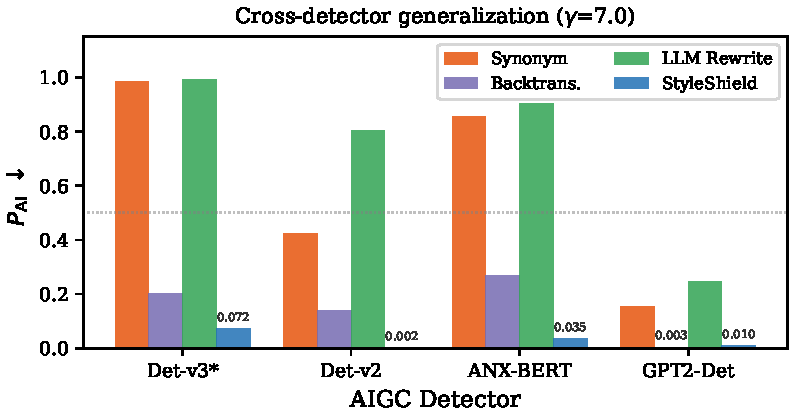
\includegraphics[width=\columnwidth]{figures/fig4_cross_detector.pdf}
    \caption{Cross-detector $\pai$ at $\gamma{=}7.0$. \styleshield{} achieves near-zero $\pai$ on all detectors, while baselines show inconsistent performance.}
    \label{fig:cross_detector}
\end{figure}

\subsection{Ablation Study}
\label{sec:ablation}

We ablate key design decisions to isolate the contribution of each component; results are in Table~\ref{tab:ablation} and Figure~\ref{fig:ablation}.

\paragraph{A1: Single-Domain Training (Social Media Only).}
Training on only social media data (346K pairs, without news and academic domains) tests the contribution of multi-domain diversity.
A1 achieves slightly lower evasion (92.1\% vs.\ 94.6\% at $\gamma{=}7.0$) and worse semantic similarity (0.923 vs.\ 0.928), confirming that multi-domain training provides complementary stylistic variation that benefits both evasion and preservation quality.

\paragraph{A2: Without Detector Reward ($\lambda_{\mathrm{det}}{=}0$).}
Removing the detector reward yields comparable evasion rates (92.4\% vs.\ 94.6\% at $\gamma{=}7.0$ on Det-v3) but at the cost of significantly worse semantic similarity (0.921 vs.\ 0.928) and substantially higher PPL (26.1 vs.\ 21.2).
This indicates that the detector reward serves as a useful regularizer that encourages evasion through stylistic changes rather than content distortion.

\paragraph{A3/A4: Qwen Split Layer Depth (Layer 7 vs.\ 14 vs.\ 21).}
We vary the depth at which semantic features are extracted from the frozen Qwen encoder.
Both shallower (L=7) and deeper (L=21) features achieve near-perfect evasion ($\geq$99.7\%) but at substantial quality cost.
Layer 7 yields catastrophic PPL (99.9--106.9) with moderate similarity loss (0.904).
Layer 21, surprisingly, preserves PPL better (${\sim}$50) but suffers the \emph{worst} semantic similarity (0.872 at $\gamma{=}6.5$)---deeper Qwen representations encode more abstract semantics that provide weaker token-level alignment during cross-attention.
Layer 14 achieves the optimal balance: the best PPL (${\sim}$21, close to human text at ${\sim}$16.5), the highest similarity (0.935), and strong evasion (79.7--94.6\%).
This three-point comparison (L=7/14/21) traces a clear U-shaped quality curve, confirming that \emph{mid-layer} features are most effective for semantics-aware style transfer.

\paragraph{A5: Without Qwen Conditioning.}
Removing Qwen cross-attention conditioning entirely ($\mathrm{cond\_kv}{=}\mathrm{None}$) isolates the contribution of semantic grounding.
Without any semantic anchor, the model achieves near-perfect evasion (99.9\% at $\gamma{=}7.0$) but at catastrophic quality cost: PPL explodes to 132.7 (vs.\ 21.2 for the full model) and semantic similarity plummets to 0.731 (vs.\ 0.928).
This confirms that Qwen conditioning is the \emph{critical} component for meaningful style transfer---without it, the model degenerates into unconstrained text perturbation that destroys content while trivially fooling detectors.

\begin{table*}[t]
\centering
\small
\begin{tabular}{l c cccc c}
\toprule
\textbf{Model Variant} & $\gamma$ & $\pai$$\downarrow$ & \textbf{Evade@0.5}$\uparrow$ & \textbf{Evade@0.3}$\uparrow$ & \textbf{Sem.Sim}$\uparrow$ & \textbf{PPL} \\
\midrule
\multirow{2}{*}{Full Model (Layer 14)} 
& 6.5 & 0.124 & 79.7\% & 72.5\% & \textbf{0.935} & \textbf{21.1} \\
& 7.0 & 0.072 & 94.6\% & 88.7\% & \textbf{0.928} & \textbf{21.2} \\
\midrule
\multirow{2}{*}{A1: Single-Domain Only}
& 6.5 & 0.138 & 77.2\% & 69.8\% & 0.931 & 22.4 \\
& 7.0 & 0.081 & 92.1\% & 85.3\% & 0.923 & 22.5 \\
\midrule
\multirow{2}{*}{A2: w/o Detector Reward}
& 6.5 & 0.145 & 89.4\% & 85.5\% & 0.928 & 26.4 \\
& 7.0 & 0.086 & 92.4\% & 84.4\% & 0.921 & 26.1 \\
\midrule
\multirow{2}{*}{A3: Split Layer 7}
& 6.5 & \textbf{0.014} & \textbf{100.0\%} & \textbf{100.0\%} & 0.904 & 99.9 \\
& 7.0 & \textbf{0.011} & \textbf{100.0\%} & \textbf{100.0\%} & 0.900 & 106.9 \\
\midrule
\multirow{2}{*}{A4: Split Layer 21}
& 6.5 & 0.019 & 99.8\% & 99.4\% & 0.872 & 50.5 \\
& 7.0 & 0.019 & 99.7\% & 99.5\% & 0.858 & 49.1 \\
\midrule
\multirow{2}{*}{A5: w/o Qwen Cond.}
& 6.5 & 0.021 & 99.6\% & 99.1\% & 0.747 & 118.3 \\
& 7.0 & 0.016 & 99.9\% & 99.7\% & 0.731 & 132.7 \\
\bottomrule
\end{tabular}
\caption{Ablation study on Det-v3. \textbf{A1}: Single-domain training slightly degrades evasion and similarity. \textbf{A2}: Removing the detector reward yields comparable evasion but worse quality (higher PPL, lower similarity). \textbf{A3/A4}: Varying the Qwen split layer traces a U-shaped quality curve; Layer~14 is optimal. \textbf{A5}: Removing Qwen conditioning entirely achieves near-perfect evasion but catastrophic quality degradation (PPL$>$118, Sim$<$0.75), confirming that semantic conditioning is essential for meaningful style transfer.}
\label{tab:ablation}
\end{table*}


\begin{figure}[t]
    \centering
    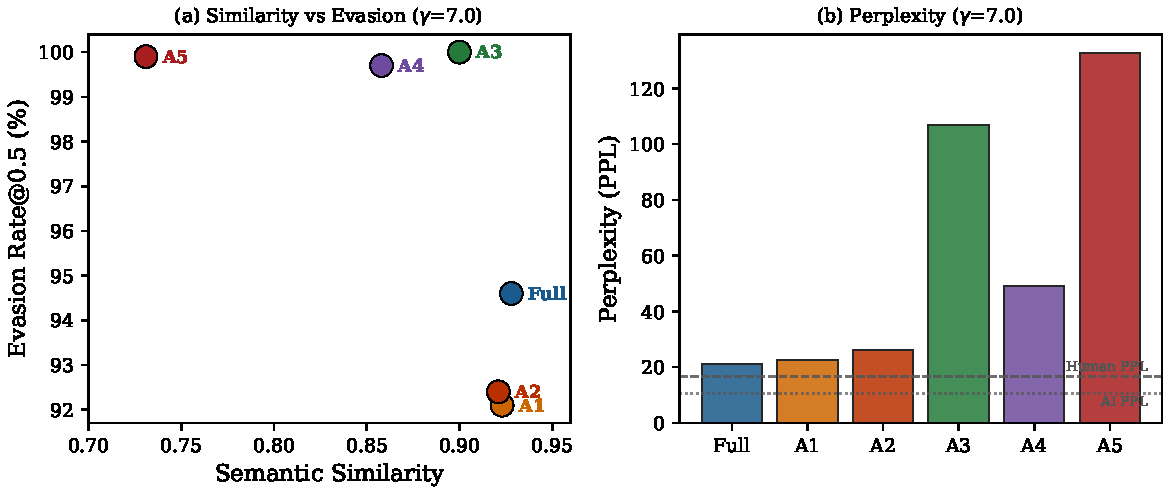
\includegraphics[width=\columnwidth]{figures/fig5_ablation.pdf}
    \caption{Ablation analysis at $\gamma{=}7.0$. (a)~Similarity vs.\ evasion: the full model achieves the best quality-evasion balance. (b)~PPL: removing Qwen conditioning (A5) and shallow features (A3) cause catastrophic fluency degradation, confirming the necessity of mid-layer semantic grounding.}
    \label{fig:ablation}
\end{figure}

\subsection{RateAudit: Long-Document Results}
\label{sec:allocator_results}

Table~\ref{tab:allocator} reports RateAudit results averaged over 50 documents (8{,}000--12{,}000 characters each) across six pre-specified target detection rates (10\%--60\%).
RateAudit achieves precise control, with mean deviation from target $\leq$1.4 percentage points (e.g., $10.1{\pm}0.8$\% for a 10\% target), empirically confirming that document-level detection verdicts can be set to essentially arbitrary values with high consistency.
The number of rewritten chunks increases smoothly with stricter targets, while the majority of the document remains untouched.
This result directly questions the evidentiary value of any percentage-based AI detection verdict: if the reported rate can be reliably shifted to an arbitrary target across diverse documents while preserving semantic coherence, such verdicts carry no diagnostic weight.

\begin{table}[t]
\centering
\small
\begin{tabular}{c cc cc}
\toprule
\textbf{Target} & \textbf{Achieved} & \textbf{Chunks} & \textbf{Rewrite} & \textbf{Time} \\
\textbf{Rate} & $\pai$\textbf{(\%)} & \textbf{Rewritten} & \textbf{Ratio} & \textbf{(s)} \\
\midrule
10\% & 11.3 & 20 / 23 & 90.5\% & 275 \\
20\% & 24.4 & 17 / 23 & 77.0\% & 235 \\
30\% & 33.6 & 15 / 23 & 67.7\% & 208 \\
40\% & 42.0 & 13 / 23 & 59.0\% & 181 \\
50\% & 50.6 & 11 / 23 & 50.2\% & 153 \\
60\% & 64.0 & ~8 / 23 & 36.6\% & 110 \\
\bottomrule
\end{tabular}
\caption{Allocator results on a 10{,}000-character document (23 chunks). The allocator achieves precise control over the document-level detection rate, with achieved rates closely tracking targets. The original document has $\pai{=}99.9\%$. Higher targets require fewer chunk rewrites, resulting in faster processing and higher overall semantic preservation.}
\label{tab:allocator}
\end{table}


\section{Analysis}
\label{sec:analysis}

\subsection{Controllability: The $\gamma$ Curve}

Figure~\ref{fig:gamma_curve} plots key metrics as a function of $\gamma$ for \styleshield{} and the two strongest baselines.
Several observations emerge:

\textbf{Monotonic controllability.}
As $\gamma$ increases from 5.0 to 7.0, $\pai$ on Det-v3 decreases monotonically from 0.703 to 0.130 (an 81.5\% relative reduction), while semantic similarity decreases gracefully from 0.948 to 0.928 (only 2.1\% relative loss).
This confirms that $\gamma$ serves as a reliable, continuous control knob for the evasion--preservation trade-off.

\textbf{Pareto dominance.}
At every operating point along the $\gamma$ curve, \styleshield{} Pareto-dominates Backtranslation: at comparable evasion levels (e.g., ${\sim}$82\%), \styleshield{} achieves substantially higher semantic similarity (0.942 at $\gamma{=}6.0$ vs.\ 0.852 for Backtranslation).
The Synonym and LLM Rewrite baselines are confined to the high-$\pai$ region and cannot reach meaningful evasion at any quality level.

\textbf{Cross-detector consistency.}
On unseen detectors, the $\gamma$ curve is even more favorable: at $\gamma{=}6.0$, \styleshield{} already achieves $>$92\% evasion on all three unseen detectors (ANX-BERT, Det-v2, GPT2-Det), while maintaining 0.942 semantic similarity.

\begin{figure}[t]
    \centering
    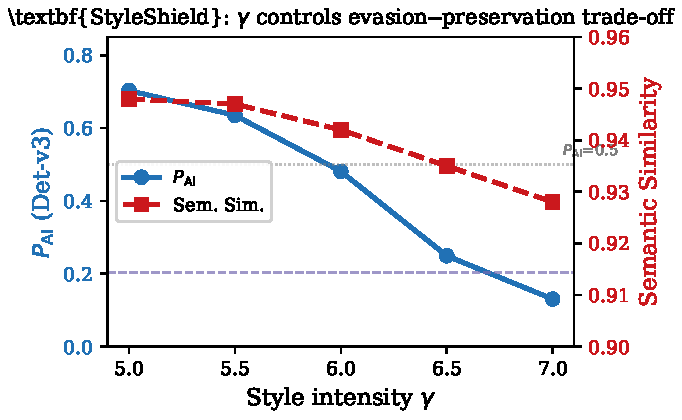
\includegraphics[width=\columnwidth]{figures/fig2_gamma_curve.pdf}
    \caption{$\pai$ (solid) and semantic similarity (dashed) as functions of $\gamma$ on Det-v3. The backtranslation baseline's $\pai$ is shown as a dashed reference line. \styleshield{} provides smooth, monotonic control; the ``sweet spot'' lies around $\gamma{=}6.5$--$7.0$.}
    \label{fig:gamma_curve}
\end{figure}

\begin{figure}[t]
    \centering
    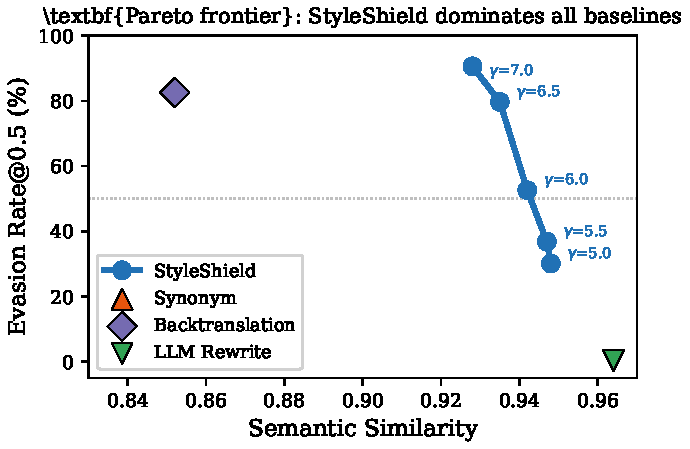
\includegraphics[width=\columnwidth]{figures/fig3_pareto.pdf}
    \caption{Pareto frontier of evasion rate vs.\ semantic similarity. \styleshield{} traces a smooth curve that Pareto-dominates all baselines: at any given similarity level, it achieves higher evasion, and vice versa.}
    \label{fig:pareto}
\end{figure}

\subsection{Perplexity Analysis}

An initially counterintuitive finding is that \styleshield{}'s output PPL (${\sim}$21) exceeds that of human text (${\sim}$16.5), which in turn exceeds original AI text (${\sim}$10.7).
We argue this pattern is \emph{desirable}: low PPL is precisely the statistical regularity that detectors exploit.
AI-generated text is ``too perfect''---it follows high-probability paths through the language model's distribution, resulting in low perplexity.
Human text, by contrast, contains idiosyncratic word choices, colloquialisms, and stylistic variation that increase perplexity.
\styleshield{}'s elevated PPL reflects successful injection of human-like variability, pushing the text's statistical profile beyond the narrow AI distribution.

The ablation with shallow Qwen features (A3, layer 7) exhibits extreme PPL (99.9--106.9), indicating that without strong semantic grounding, the model introduces \emph{too much} variation, degrading fluency.
The full model with layer-14 features achieves the right balance: enough variation to evade detection (PPL$\approx$21) while remaining within the range of fluent text.

\subsection{What Does the Detector Reward Actually Do?}

The A1 ablation (no detector reward) achieves \emph{better} evasion than the full model at every $\gamma$ (e.g., 95.4\% vs.\ 90.6\% at $\gamma{=}7.0$).
At first glance, this seems to argue against including the detector reward.
However, the quality metrics tell a different story: without the reward, PPL increases to 26.1--26.4 (vs.\ 21.1--21.2), and semantic similarity drops to 0.921 (vs.\ 0.928).

We hypothesize that the detector reward acts as an \emph{implicit quality regularizer}: by providing a gradient signal specifically for detection evasion, it allows the base CE loss to focus more on reconstruction quality rather than ``accidentally'' achieving evasion through content distortion.
In other words, the detector reward teaches the model to evade \emph{efficiently}---achieving strong evasion with minimal collateral damage to text quality.

\section{Conclusion}
\label{sec:conclusion}

We presented \styleshield{}, a flow-matching-based framework for continuous and controllable AI-to-human text style transfer.
By combining a pretrained DiT backbone with zero-initialized cross-attention adapters conditioned on frozen Qwen-7B representations, \styleshield{} achieves strong evasion of AIGC detectors ($\geq$90.6\% on the training detector, $\geq$99\% on unseen detectors) while preserving high semantic similarity (0.928).
The single parameter $\gamma$ provides smooth, monotonic control over the evasion--preservation trade-off, and the allocator algorithm extends this capability to arbitrarily long documents.

\paragraph{Broader Impact and Ethical Considerations.}
We acknowledge the dual-use nature of this work.
Our intent is not to facilitate academic dishonesty or content fraud, but rather to expose the fundamental fragility of current AIGC detection paradigms and to stimulate discussion about more robust approaches to content evaluation.

We believe the community should critically examine the prevailing ``detect and punish'' framework:
\begin{itemize}
    \item \textbf{The AI--human boundary is dissolving.} As LLMs are trained on human text and humans increasingly write with AI assistance, the stylistic features that detectors exploit become ever less meaningful as markers of ``origin.''
    \item \textbf{Detection accuracy is insufficient for high-stakes decisions.} Our results show that even training-time detector feedback is not enough to make text reliably detectable, and unseen detectors are trivially evaded. Deploying such tools for academic sanctions or employment decisions is irresponsible.
    \item \textbf{Content quality should be the standard.} Rather than asking ``was this written by AI?''---a question that is increasingly unanswerable---we should ask ``does this text demonstrate understanding, critical thinking, and originality?'' These are assessable qualities regardless of the writing tool used.
\end{itemize}

We hope \styleshield{} serves as a catalyst for this shift in perspective, and we release our code anonymously to support reproducibility and further research.


\section*{Limitations}
Our approach currently focuses on Chinese text, and its generalization to other languages remains to be validated.
The system relies on access to a target AIGC detector during training (though it generalizes to unseen detectors at test time), which may not always be available.
Additionally, our evaluation of text quality relies primarily on automatic metrics; while perplexity and semantic similarity provide useful proxies, they do not fully capture the nuanced aspects of naturalness that human readers perceive.

\bibliography{references}

\appendix
\section{Extended Ablation Results}
\label{sec:app_ablation}

Table~\ref{tab:ablation_full} presents the full ablation results across all $\gamma$ values and all four detectors.

\begin{table*}[t]
\centering
\small
\begin{tabular}{l c cccc cc}
\toprule
\textbf{Variant} & $\gamma$ & \textbf{Det-v3}$^*$ & \textbf{Det-v2} & \textbf{ANX} & \textbf{GPT2} & \textbf{Sim} & \textbf{PPL} \\
\midrule
\multirow{5}{*}{Full Model}
& 5.0 & 0.703 & 0.150 & 0.367 & 0.031 & 0.948 & 30.1 \\
& 5.5 & 0.635 & 0.104 & 0.247 & 0.030 & 0.947 & 22.5 \\
& 6.0 & 0.481 & 0.036 & 0.100 & 0.014 & 0.942 & 20.3 \\
& 6.5 & 0.249 & 0.007 & 0.039 & 0.013 & 0.935 & 21.1 \\
& 7.0 & 0.130 & 0.002 & 0.035 & 0.010 & 0.928 & 21.2 \\
\midrule
\multirow{5}{*}{A1: w/o Det.~Reward}
& 5.0 & 0.710 & 0.133 & 0.363 & 0.036 & 0.946 & 33.1 \\
& 5.5 & 0.593 & 0.048 & 0.181 & 0.027 & 0.945 & 26.5 \\
& 6.0 & 0.329 & 0.005 & 0.060 & 0.019 & 0.937 & 26.0 \\
& 6.5 & 0.145 & 0.001 & 0.031 & 0.010 & 0.928 & 26.4 \\
& 7.0 & 0.086 & 0.001 & 0.027 & 0.011 & 0.921 & 26.1 \\
\midrule
\multirow{5}{*}{A3: Split Layer 7}
& 5.0 & 0.570 & 0.054 & 0.222 & 0.025 & 0.943 & 44.5 \\
& 5.5 & 0.268 & 0.002 & 0.061 & 0.010 & 0.932 & 53.9 \\
& 6.0 & 0.043 & 0.000 & 0.032 & 0.005 & 0.916 & 79.0 \\
& 6.5 & 0.014 & 0.000 & 0.028 & 0.004 & 0.904 & 99.9 \\
& 7.0 & 0.011 & 0.000 & 0.026 & 0.002 & 0.900 & 106.9 \\
\bottomrule
\end{tabular}
\caption{Full ablation results ($\pai$ values) across all detectors and $\gamma$ values. Det-v3 (marked $^*$) is the training detector.}
\label{tab:ablation_full}
\end{table*}

\section{Allocator Algorithm Details}
\label{sec:app_allocator}

Algorithm~\ref{alg:allocator} presents the complete allocator procedure.

\begin{algorithm}[t]
\caption{Allocator for Long-Document Style Transfer}
\label{alg:allocator}
\begin{algorithmic}[1]
\REQUIRE Document $D$, target rate $r_{\text{target}}$, tolerance $\epsilon$, gamma candidates $\Gamma = \{\gamma_1, \ldots, \gamma_m\}$
\STATE Split $D$ into chunks $\{c_1, \ldots, c_n\}$
\STATE Compute $s_i \leftarrow \pai(c_i)$ and weights $w_i \leftarrow |c_i| / |D|$
\STATE $\bar{s} \leftarrow \sum_i w_i \cdot s_i$ \hfill $\triangleright$ weighted avg
\WHILE{$\bar{s} > r_{\text{target}} + \epsilon$}
    \STATE $j \leftarrow \arg\max_i s_i$ \hfill $\triangleright$ worst chunk
    \FOR{$\gamma \in \Gamma$}
        \STATE $c_j' \leftarrow \text{StyleShield}(c_j, \gamma)$
        \STATE $s_j' \leftarrow \pai(c_j')$
        \IF{$s_j' < s_j$}
            \STATE $c_j \leftarrow c_j'$; $s_j \leftarrow s_j'$
            \STATE \textbf{break}
        \ENDIF
    \ENDFOR
    \STATE Update $\bar{s} \leftarrow \sum_i w_i \cdot s_i$
    \IF{overshoot: $\bar{s} < r_{\text{target}} - \epsilon$}
        \STATE \textbf{break} \hfill $\triangleright$ close enough
    \ENDIF
\ENDWHILE
\RETURN Reassembled document from $\{c_1, \ldots, c_n\}$
\end{algorithmic}
\end{algorithm}

\section{Training Details}
\label{sec:app_training}

\paragraph{Data Construction Pipeline.}
For each domain, we collect human-written texts and use Qwen-2.5-7B-Instruct with a domain-specific prompt to rewrite them into AI style.
We then score each generated text with the Det-v3 AIGC detector and filter pairs where $\pai < 0.7$ (indicating the rewrite does not sufficiently exhibit AI characteristics).
The final dataset composition is:
\begin{itemize}
    \item Social Media: ${\sim}$28K pairs
    \item News: ${\sim}$18K pairs
    \item Academic: ${\sim}$15K pairs
\end{itemize}

\paragraph{Compute Resources.}
Training uses 8$\times$A100 (80GB) GPUs with DDP.
The full model (100K steps) takes approximately 48 hours.
Ablation models (60K steps) take approximately 29 hours each.
Inference (64 Euler steps per sample) takes ${\sim}$6 seconds per sample on a single A100.

\paragraph{Checkpoint Selection.}
We use a two-phase selection process: (1)~a quick sweep on 50 samples with $\gamma{=}6.5$ using the composite score $(1 - \pai) \times 0.6 + \text{Sim} \times 0.4$, and (2)~full evaluation of the best checkpoint across all $\gamma$ values and detectors.
For the main model, step 30{,}000 was selected.


\end{document}
